\documentclass{article}
\usepackage{graphicx, appendix, array, listings}
\renewcommand{\appendixpagename}{Appendix}

\graphicspath{ {./img/} }

% Title page
\title{Report Rascal Assignment}
\author{Bas van de Louw, Brent Van Handenhove}
\date{15-Jan-2022}

\begin{document}
\maketitle

\begin{table}[h!tbp]
	\caption{Team}
	\begin{tabular}{l|l}
		\hline
		Bas van de Louw      & 852361065 \\
		\hline
		Brent Van Handenhove & 852152619 \\
		\hline
	\end{tabular}
\end{table}

\hrulefill{}

\vfill
\clearpage

%TOC page
\tableofcontents
\vfill
\clearpage

\section{Design}

\subsection{Assumptions made}

\subsubsection{Only considering Java files}
We will only be counting Java source files. Any compiled Java code or code written in another language is ignored.

\subsubsection{What is a 'Line of Code'} \label{defining loc}
In order to calculate the total amount of code or unit size, we have to first define what a 'line of code' is.

For the purpose of this project, we decided that a line should check all the below rules for it to be considered a line of code:

\begin{itemize}
\item Not blank: Trimmed length of line is 0
\item Not a comment: Starts with //, /*, * or ends with */
\end{itemize}

One caveat here is that in Java, lines of legitimate code may actually start with * as seen below:
\begin{lstlisting}
      int x=10;
      int y=25;
      int z=x
      *
      y;
\end{lstlisting}

However, this is usually code smell except in rare complex mathematical calculations (of which there are none in either project). For this assignment, we will assume code should not have this. We assume that no non-comment lines will start with *.
In a real life scenario, as illustrated above, it may happen. As such, a more mature analysis tool should handle this more appropriately.

Some additional things to consider are:
\begin{itemize}
\item Our program was run on Windows - any variations on Linux and Mac may be due to differences in how the OS handles text. 
\item There was no style normalization, the project was analysed 'as is'.
\end{itemize}

In addition, we count the import of other modules as lines of code. We also count the module declaration itself as a line of code. Whether or not these are really lines of code can be debated. We have decided that they are, as they are essential for the code to function.

\subsubsection{Lines of Code}
In addition to the assumptions and caveats in \ref{defining loc}, we have noticed that Eclipse tends to generate some additional files for the SmallSQL / HSQLDB projects that may affect our metrics. For example: The amount of lines of code for SmallSQL increases by roughly 2000 when this happens.
For the rest of this report, assume that we have discarded any generated files and are looking solely at the base project.

The pseudo-code for determining the total lines of code in a project is as follows:
\begin{enumerate}
\item Get all java files in a project
\item For each file
\subitem Count the amount of lines that are not blank and not a comment
\end{enumerate}

This means we also count each of these as a line of code:
\begin{itemize}
\item Test code (as long as it is in Java)
\item Single-line curly brackets
\end{itemize}

\subsubsection{Unit Count}
SIG defines a unit as 'the smallest named piece of executable code'
Every implemented method within the project is counted towards the total unit count. As such, we can define the unit count as the amount of implemented methods within the project. Methods without an implementation are discarded, as they are not executable.

The pseudo-code for determining unit size is as follows:
\begin{enumerate}
\item Get the project AST
\item For each node
\subitem Check if it is a method with an implementation (so that it is executable)
\subitem If so, increment the unit count
\end{enumerate}

\subsubsection{Unit Size}
Each unit within the project has a size. We calculate the size as the amount of lines of code within the unit that check the requirements set in \ref{defining loc}. Note that the caveats apply here as well and that we also count single-line curly brackets.

\subsubsection{Unit Complexity}
Each unit within the project has a cyclomatic complexity. The complexity of unit is equal to the  sum of the complexity of each statement within the unit plus 1. Each statement within table \ref{complexityvalues} increases the unit complexity by a value of 1.

We do not count the complexity of invoked methods towards the complexity of a method. This would not make sense, as the metric is supposed to be used to estimate which methods could be broken up into smaller methods.

\begin{table}[h!tbp]
	\caption{Cyclomatic Complexity Statements}
	\label{complexityvalues}
	\begin{tabular}{l|l}	
		\hline
		if(\_, \_)					&			if statement \\
		\hline
		case(\_)					&			case within a switch \\
		\hline
		do(\_, \_)					&			do loop \\
		\hline
		while(\_,\_)				&			while loop \\
		\hline
		for(\_, \_, \_)				&			for loop \\
		\hline
		foreach(\_, \_, \_)			&			foreach loop \\
		\hline
		catch(\_, \_)				&			catch statement \\
		\hline
		conditional(\_, \_, \_)		&			conditional \\
		\hline
		infix(\_, "\&\&", \_)		&			infix AND \\
		\hline
		infix(\_, "\(||\)", \_)		&			infix OR \\
		\hline
	\end{tabular}
\end{table}

\subsubsection{Duplication} \label{dupereqs}
For code to be considered duplicate, it has to check the following requirements:
\begin{itemize}
\item The node tree should have at least 25 nodes (see below)
\item The location of the code cannot be unknown (see below)
\item It has to be at least 6 lines long (see \ref{defining loc})
\end{itemize}

We insist the node tree has to be at least 25 nodes long (declarations, statements or expressions all count towards this number). This helps us weed out any code that we deem too small to be an issue, such as simple calculations or getters/setters. While most of these wouldn't check the 6-line-minimum, it's still possible to spread very simple code over many lines (see caveat at \ref{defining loc})

Code with an unknown location is discarded, as it is impossible for us to verify that we are not checking the same code twice if our algorithm finds it identical to other code.

There are some additional rules we have established within our metric:
\begin{itemize}
\item By ignoring method and argument types, code may be marked as duplicate where it does in fact make sense to have similar implementations. We are aware of these possible false-positives and accept this risk.
\item Only exact matches (after discarding types) are considered. It is possible to check for near-misses and mark them as well, but we have decided not to do that for this project.
\item Duplicate code is counted on a unique occurrence basis, meaning if there are 3 chunks of duplicate code we count 3 of them as duplicate.
\item Code marked as duplicate that is part of a larger chunk of code marked as duplicate is discarded. This prevents us from counting so-called 'sub-clones' towards the total amount of duplicate code, as this would effectively count some code twice.
\end{itemize}

The pseudo-code for our duplication metric is presented below.

\begin{enumerate}
\item For every node in the AST
\subitem If the location is valid (not unknown and at least 6 lines of code)
\subitem Normalize the node (remove all return types, method types, literal values) for comparison
\subitem Check if this exact node (loc) was not already tracked to prevent literal identical duplicates
\subitem If it is not an identical match, it is a clone - add it to the list with the node as key
\item Do a pass over the list of detections and remove any nodes where there are not at least 2 values in the list (which would indicate there are no duplicates)
\end{enumerate}

By default, we also prune what we call 'subclones'. These are bits of code marked as duplicate that are also part of a larger bit of code that is also marked as duplicate. If we didn't perform this, we would be counting these twice. This can happen because the AST is evaluated per-node instead of per-method. While this allows us to pick up duplicate code inside of methods as well as duplicate method declarations, it does mean we treat code inside a method as a separate thing to check.
Here is how pruning works:

\begin{enumerate}
\item Do a runtime pass is done to check if duplicate code is not part of a larger chunk of duplicate code to avoid counting the same code twice
\item Do a second pass is done after all duplicate code has been checked in so that a 'subclone' added before its larger clone (which would not be picked up during our previous pass) is also not counted
\end{enumerate}

\subsubsection{Test Coverage} \label{assumetests}
In order to calculate test coverage, some likely inaccurate assumptions were made.
Primarily, we do not check for any 'real' unit testing that may be present - such as JUnit - because we can neither rely on assuming one test library is used nor can we account for any unknown or proprietary test libraries. In addition, any Rascal locations that point to an outside library do not appear to be tracked.

To explain our process for calculating test coverage, we go through the following steps in pseudo code:

\begin{enumerate}
\item Create a list of every method (=unit) and its location in the project
\item Create two empty lists for 'real' methods and 'test' methods
\item For every method
	\begin{enumerate}
	\item If it contains at least 1 assert, add it to the list of test methods
	\item If it has no asserts and the access modifier is public, add it to the list of real methods
	\end{enumerate}
\item Create an empty list for 'covered' methods
\item For every method in test methods
	\begin{enumerate}
	\item Get every method called within the test method
	\item If they are not yet in the list for covered methods, add them
	\end{enumerate}
\item The amount of covered methods divided by the amount of 'real' methods is the test coverage percentage
\end{enumerate}

You may have noticed that we are only counting public methods. This is because we assume that private methods are either:

\begin{itemize}
\item Used within a public method (and thus indirectly tested)
\item Only used internally (and thus not of any interest to us)
\end{itemize}

We make an additional assumption in that we count every method call that follows the pattern \verb|'/^assert/i'| as an assert. In doing this, we implicitly assume the following:
\begin{itemize}
\item That every asserting method's name starts with 'assert' (e.g. assert, assertEquals, assertNull, etc)
\item That any other method's name does not start with 'assert'.
\end{itemize}

Lastly, we do not perform a final check to ensure every covered method is public. This is because we assume that unit tests are not within the same file or package, so they should not be able to access anything other than public methods.

\subsection{Visualizing the data}
Table~\ref{results} shows the computed metrics, which provide us a solid overall picture of the maintainability state of the evaluated projects.
When visualizing this data we wanted to give an insight on how to fix these maintainability issues. 
For this reason we chose a fine-grained view, so that issues can be traced back to their source.

\subsubsection{Using fine-grained views}
We began by designing a menu to let users traverse the available projects.
Then, for unit sizes, cyclomatic complexity, and duplication, we introduced three fine-grained views.
Risk factors can be used to filter these views to an even more detailed view.
We can, for example, limit the cyclomatic complexity visualization to units with a cyclomatic complexity greater or equal to 50.
Software Improvement Group (SIG)~\cite{SIG} considers this code to be untestable and a very high risk.

Because the goal is to eventually fix these issues, we made these views interactive.
Clicking on a unit in any fine-grained view will cause the visualization to open a new tab with the source code location.
This makes locating the root of major maintainability problems a simple task.
Appendix~\ref{appendix:visualization} contains further information on the fine-grained views.

\section{Results}

\subsection{Metrics}
The calculated metrics for SmallSQL and HSQLDB can be found in table \ref{results}.

\begin{table}[!htb]
\caption{Metric results}
\label{results}
\begin{minipage}{.5\linewidth}
\caption{SmallSQL}
\centering
\begin{tabular}{l|r}	
		\multicolumn{2}{c}{General Data}		\\		
		\hline
		Lines of Code			&			24 850 \\
		\hline
		Number of Units			&			2 358 \\
		\hline
		
		\noalign{\vskip 4mm}    
		\multicolumn{2}{c}{Unit Size}		\\					 
		\hline
		Simple					&			38.1 \% \\
		\hline
		Moderate				&			15.0 \% \\
		\hline
		High					&			20.5 \% \\
		\hline
		Very High				&			26.3 \% \\
		\hline
		
		\noalign{\vskip 4mm}    
		\multicolumn{2}{c}{Unit Complexity}		\\					 
		\hline
		Simple					&			63.0 \% \\
		\hline
		Moderate				&			10.6 \% \\
		\hline
		High					&			16.9 \% \\
		\hline
		Very High				&			9.5 \% \\
		\hline		
		
		\noalign{\vskip 4mm}    
		\multicolumn{2}{c}{Duplication}		\\					 
		\hline
		Duplication				&			15.5 \% \\
		\hline
		
		\noalign{\vskip 4mm}    
		\multicolumn{2}{c}{Unit Testing}		\\					 
		\hline
		Coverage				&			29.6 \% \\
		\hline
		Asserts					&			961 \\
		\hline
				
		\noalign{\vskip 4mm}    
		\multicolumn{2}{c}{Metric Scoring}		\\					 
		\hline
		Unit Size Score			&			- - \\			 
		\hline
		Volume Score			&			+ + \\			 
		\hline
		Unit Complexity Score	&			- - \\			 
		\hline
		Duplication Score		&			- \\			 
		\hline
		Unit Testing Score		&			- \\
		\hline
		
		\noalign{\vskip 4mm}    
		\multicolumn{2}{c}{SIG Scoring}		\\					 
		\hline
		Analyzability			&			o \\
		\hline
		Changeability			&			- \\
		\hline
		Stability				&			- \\
		\hline
		Testability				&			- - \\
		\hline
		Overall Maintainability &			- \\ 		
		\hline
\end{tabular}
\end{minipage}%    
\begin{minipage}{.5\linewidth}
\centering
\caption{HSQLDB}
\begin{tabular}{l|r}	
		\multicolumn{2}{c}{General Data}		\\		
		\hline
		Lines of Code			&			160 929 \\
		\hline
		Number of Units			&			9 424 \\
		\hline
		
		\noalign{\vskip 4mm}    
		\multicolumn{2}{c}{Unit Size}		\\					 
		\hline
		Simple					&			19.8 \% \\
		\hline
		Moderate				&			16.8 \% \\
		\hline
		High					&			20.6 \% \\
		\hline
		Very High				&			42.9 \% \\
		\hline
		
		\noalign{\vskip 4mm}    
		\multicolumn{2}{c}{Unit Complexity}		\\					 
		\hline
		Simple					&			59.9 \% \\
		\hline
		Moderate				&			16.4 \% \\
		\hline
		High					&			13.4 \% \\
		\hline
		Very High				&			10.4 \% \\
		\hline		
		
		\noalign{\vskip 4mm}    
		\multicolumn{2}{c}{Duplication}		\\					 
		\hline
		Duplication				&			19.6 \% \\
		\hline
		
		\noalign{\vskip 4mm}    
		\multicolumn{2}{c}{Unit Testing}		\\					 
		\hline
		Coverage				&			6.0 \% \\
		\hline
		Asserts					&			691 \\
		\hline
				
		\noalign{\vskip 4mm}    
		\multicolumn{2}{c}{Metric Scoring}		\\					 
		\hline
		Unit Size Score			&			- - \\			 
		\hline
		Volume Score			&			+ \\			 
		\hline
		Unit Complexity Score	&			- - \\			 
		\hline
		Duplication Score		&			- \\			 
		\hline
		Unit Testing Score		&			- - \\
		\hline
		
		\noalign{\vskip 4mm}    
		\multicolumn{2}{c}{SIG Scoring}		\\					 
		\hline
		Analyzability			&			- \\
		\hline
		Changeability			&			- \\
		\hline
		Stability				&			- - \\
		\hline
		Testability				&			- - \\
		\hline
		Overall Maintainability &			- \\ 		
		\hline
\end{tabular}
\end{minipage} 
\end{table}

\subsection{Interpreting the results}
\subsubsection{Lines of Code}

\subsubsection{Unit Size}

\subsubsection{Unit Complexity}
\subsubsection{Duplication}

\subsubsection{Test Coverage}


\section{Evaluation and Reflection}

\subsection{Validity}

\subsubsection{Lines of Code} \label{validloc}
We added unit testing for our project volume calculation metric, which also affects \ref{validunitsize}.These verify that our metric is accurate by our own defined rules in \ref{defining loc}. 
Our unit test below checks for our defined requirements and returns '18', which is the expected amount.

\begin{lstlisting}
package unit_tests.resources;

public class VolumeExampleTest {
	
	public static String test1() {
		return "test1";
	}
	
	/**
	 * This comment should not be counted
	 * 
	 * @return A string
	 */
	public static String test2() {
		return "test2";
	}
	
	/*
	 * Ignore
	 */
	public static int test3() {
		int a = 1;
		int b = 1;
		return a;
	}
	
	// Not a valid JavaDoc and should not be counted towards volume
	public static int test4() {
		int a = 1;
		return a;
	}
}
\end{lstlisting}

An additional, extremely rudimentary way of checking if our result is realistic is by taking the total file size of all source files and dividing it by the average size of a line of code. If we put the average line of code at 50 bytes (or 50 characters), we come to a result of 26 662 for SmallSQL, which matches our metrics.

To get to our average, we took the file 'SSResultSet.java' within SmallSQL, calculated the amount of characters and divided it by the amount of lines. This was a total of 36 759 characters over 1 280 lines (including blanks and comments). This resulted in an average characters/line of 28.7. Rounding up to 30 brings us to 44 437 lines. If we discard comments (5 105) and blank lines (658) we are at 30 996 characters over 903 lines, or roughly 34 characters/line. This brings us to 38 000 lines of code. This margin of almost 50\% above our estimated amount seems excessive, but given that some files are almost 40\% comments (such as LongTreeList.java) it is reasonable to assume that this is plausible.

\subsubsection{Unit Size} \label{validunitsize}
The unit test applied for lines of code (see \ref{validloc}) is also relevant here.

We recognize that not counting comments, while more accurate for the metric, may lead to situations where methods are overly documented. Whilst poorly documented code is harder to understand, overly documented code may also be harder to understand.

We think this is something that should either be included in the unit size calculation somehow, or that a separate metric should be created to indicate overly documented code. Any amount of comments over a certain threshold could be seen as 'too much'. We have not applied this idea in our metrics for this project.

\subsubsection{Unit Complexity}
We wrote unit tests to ensure our unit complexity metric is accurate. The expected results for the unit tests below are 2 and 4 respectively, which is what our metric reports. This indicates that we implemented it correctly

\begin{lstlisting}
public static String test1() {
	int x = 0;
	if(x == 0) {
		x++;
	}
	return "test";
}

public static String test2() {
	int x = 0;
	int y = 1;
	if(x == 0) {
		x++;
	}
	while(x == 1) {
		if(y == 10)
		{
			x++;
		}
		else {
			y++;
		}
	}
	return "test";
}
\end{lstlisting}

We also performed some manual checks on SmallSQL files by cross-referencing the reported complexity by our metric with a manual calculation of the expected result. Whenever we did this, the expected result would match our output.

\subsubsection{Duplication}
By ignoring method and argument types, code may be marked as duplicate where it could make sense to have similar implementations.

Let's take a look at an example from SmallSQL:

\begin{lstlisting}
public Date getDate(int i) throws SQLException {
    try{
		Expression expr = getValue(i);
        wasNull = expr.isNull();
		if(wasNull) return null;
		return DateTime.getDate( expr.getLong() );
    }catch(Exception e){
        throw SmallSQLException.createFromException( e );
    }
}
public Time getTime(int i) throws SQLException {
    try{
		Expression expr = getValue(i);
        wasNull = expr.isNull();
		if(wasNull) return null;
		return DateTime.getTime( expr.getLong() );
    }catch(Exception e){
        throw SmallSQLException.createFromException( e );
    }
}
\end{lstlisting}

Because our duplication-check ignores method return types, it will mark these methods as duplicate, as they check the requirements in \ref{dupereqs}. 
There are likely cleaner ways to handle code such as this (because admittedly, it is almost identical), but we realize that it is not always pragmatic to do so. 

For the example method above, though, the getValue() and null-check segment could have been split into a different method - so in this case, we are fine marking it as duplicate.

More false-positives happen especially when dealing with localization. SmallSQL, for example, contains a localization template and 3 language files, all as java files. We ignore the contents of strings, so all language files are marked as duplicate. This makes sense, as they will all use the same keys for localization purposes. This means these are false-positives and will skew results towards a higher duplication estimate.

Having said that, we propose that having localization files as java files is bad practice and should have been handled using files specifically made to handle data (such as json or csv).

\subsubsection{Unit Test Coverage}
Something we wanted to do but couldn't was to verify that the assert decl was inside of a test library. We could do this by checking if, for example, 'junit.org' was inside the decl path. However, it appears Rascal does not correctly handle a decl to an outside library. Instead, they are 'unknown', meaning this additional check we wanted to do was not possible at this time. This means any 'assert'-named method that is not an actual assert/test will violate our assumption in \ref{assumetests} but will not be caught. This means it will count as a test method and could skew results towards a higher coverage.

Another limitation to using our method of estimating test coverage is that 'partial tests' are not properly handled. What we mean with this is that test methods that by themselves do not contain an assert are not evaluated, even if they are called by another test method that does contain asserts. Likewise, a test method with an assert that does not itself invoke the methods it tests are not properly handled.
In other words, we do not support nested testing. This may skew results towards a lower coverage.

We can conclude that while we believe our method of calculating test coverage is at worst an educated guess and at best an acceptable estimation.

\subsection{Evaluating the visualisation}

\subsection{Cooperation}
\subsubsection{Working as a team}
Having worked together before, we knew each other's strengths and weaknesses. Even though we both work full-time, we constantly communicated about ideas, questions, and specific code implementations. 
In the evenings, we would each work on different parts of the code - often sending over what we were currently working on for quick feedback. This allowed us to implement features quickly while having a form of code reviews.

\subsubsection{Version control}
To ease collaboration, we used git for this project.

After we had a good foundation, we started using pull requests for further features and bug fixes. We did not do this right away as we do not believe it fruitful to complicate the pipeline so early into development. We found that this works well for us.

There were constant code reviews, mostly informal due to the small team size.

\subsubsection{Work division}
No specific work division was done, as neither of us had any experience with Rascal. It is our belief that on a project of smaller scope with a small team, working on a bit of everything leads to a better result.

\begin{table}[h!tbp]
	\caption{Work division}
	\begin{tabular}{l|l}
		\hline
		Bas van de Louw      & Design, code, report \\
		\hline
		Brent Van Handenhove & Design, code, report \\
		\hline
	\end{tabular}
\end{table}

% References 
\bibliographystyle{IEEEtran}
% your references should be in the file ref.bib
\bibliography{IEEEabrv,ref}

\clearpage
\appendix
\appendixpage{}

\section{Visualization}
\label{appendix:visualization}
\subsection{Menu}
Menu containing a project selector and analysis tool.
\begin{figure}[!htbp]
	\centering
	\label{fig:vis-menu}
	\caption{Menu}
	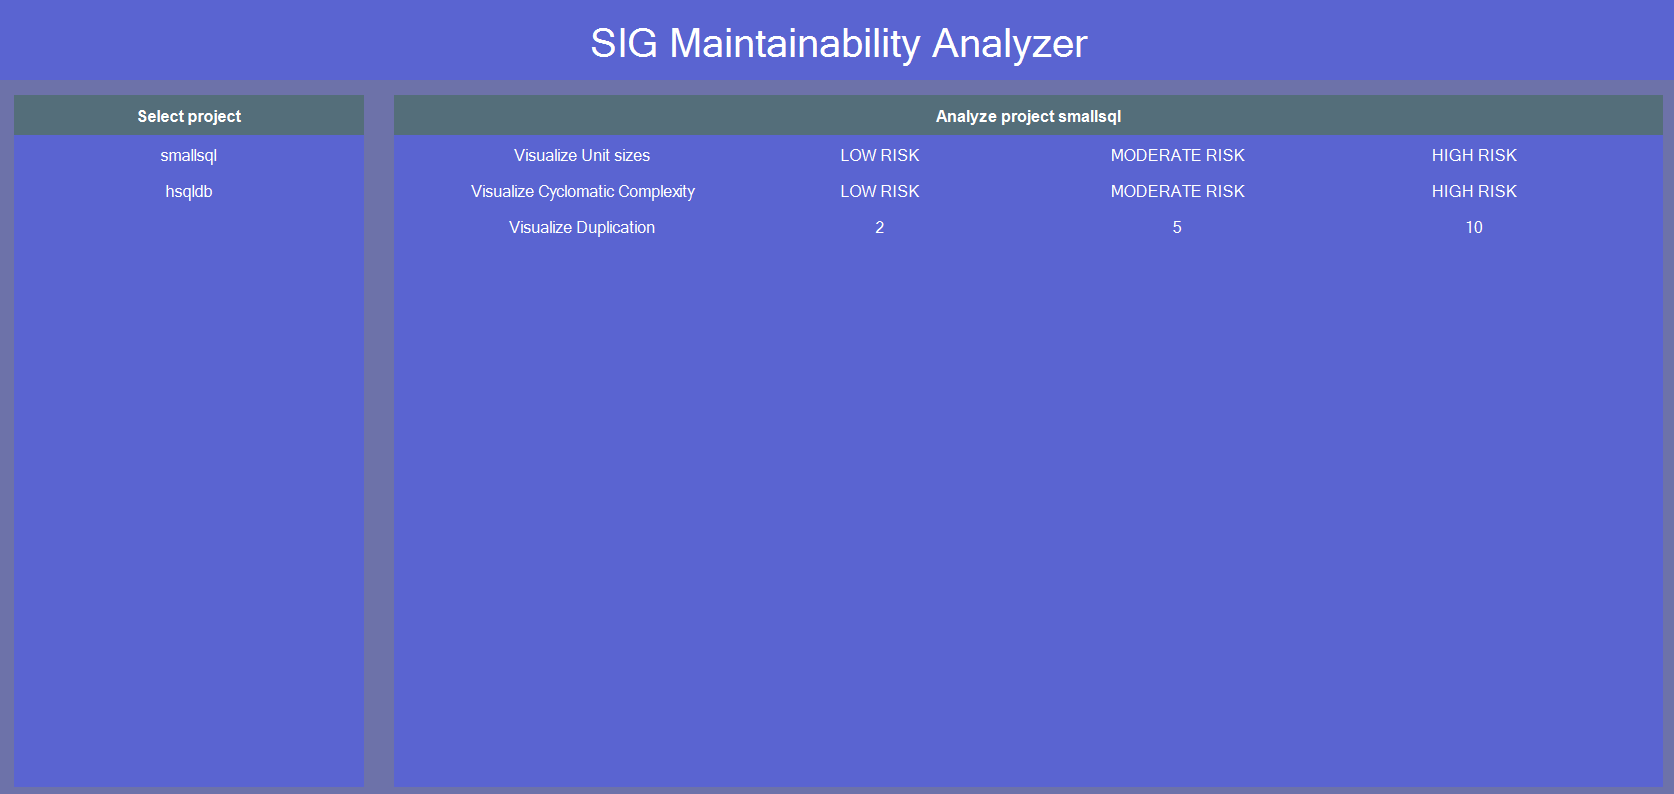
\includegraphics[width=400px, height=200px]{vis_menu.png}
\end{figure}

\subsection{Fine-grained views}
For every fine-grained view, the same concept applies. 
The user can hover over a unit and then the file, path and lines of code (loc) will be displayed on screen. 
Additionally, the user can click on the unit and a new window will be opened where the source code is located.
In below fine-grained view of high risk units (loc 40+) from the HSQLDB project we can easily see that the biggest unit has a size of 872. 

\begin{figure}[!htbp]
	\centering
	\label{fig:unit-sizes}
	\caption{Fined grained view high-risk HSQLDB: Unit sizes}
	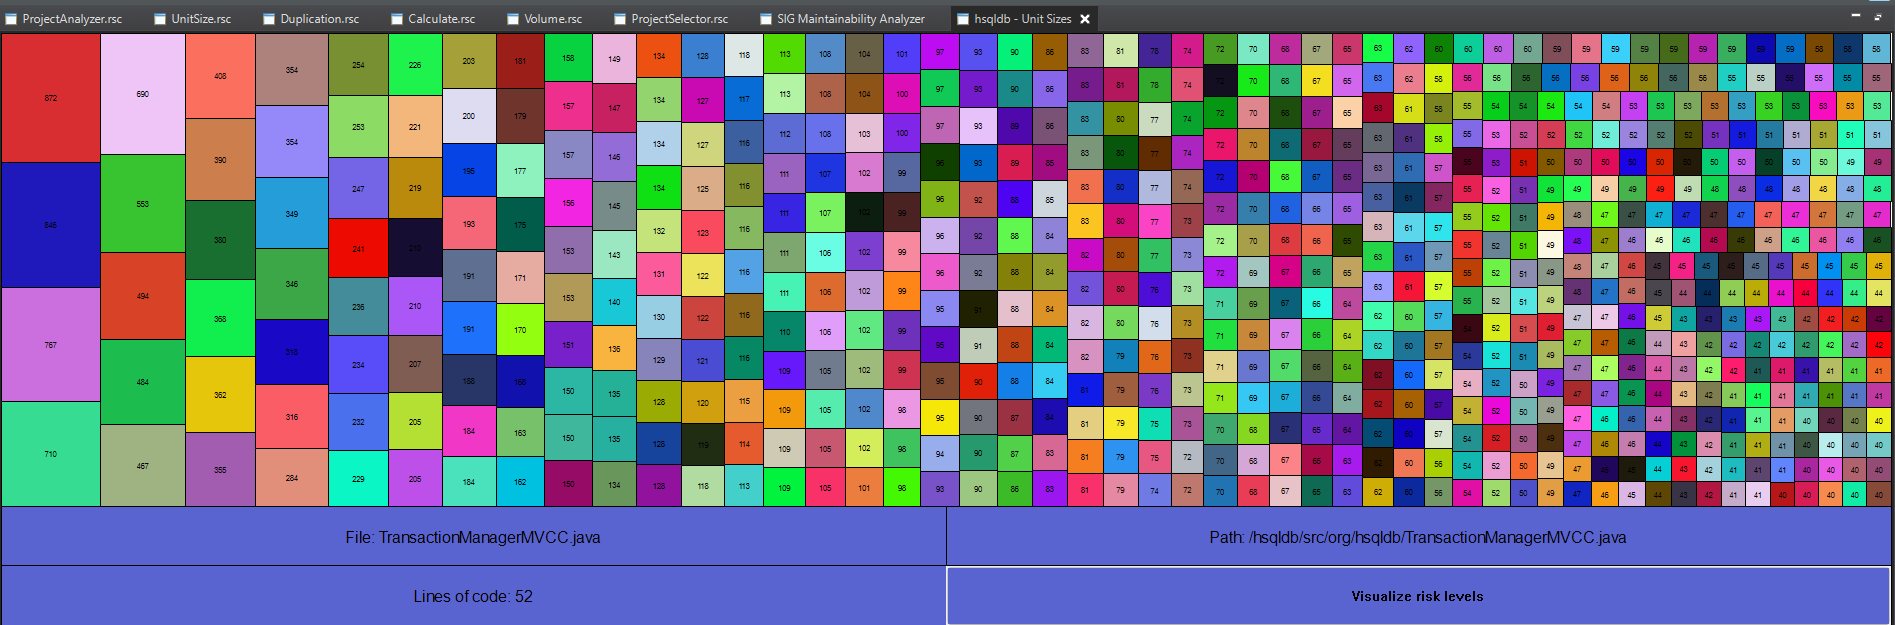
\includegraphics[width=400px, height=200px]{hsqldb_unitsizes.png}
\end{figure}

\begin{figure}[!htbp]
	\centering
	\label{fig:cyclomatic-complexity}
	\caption{Fined grained view high-risk HSQLDB: Cyclomatic complexity}
	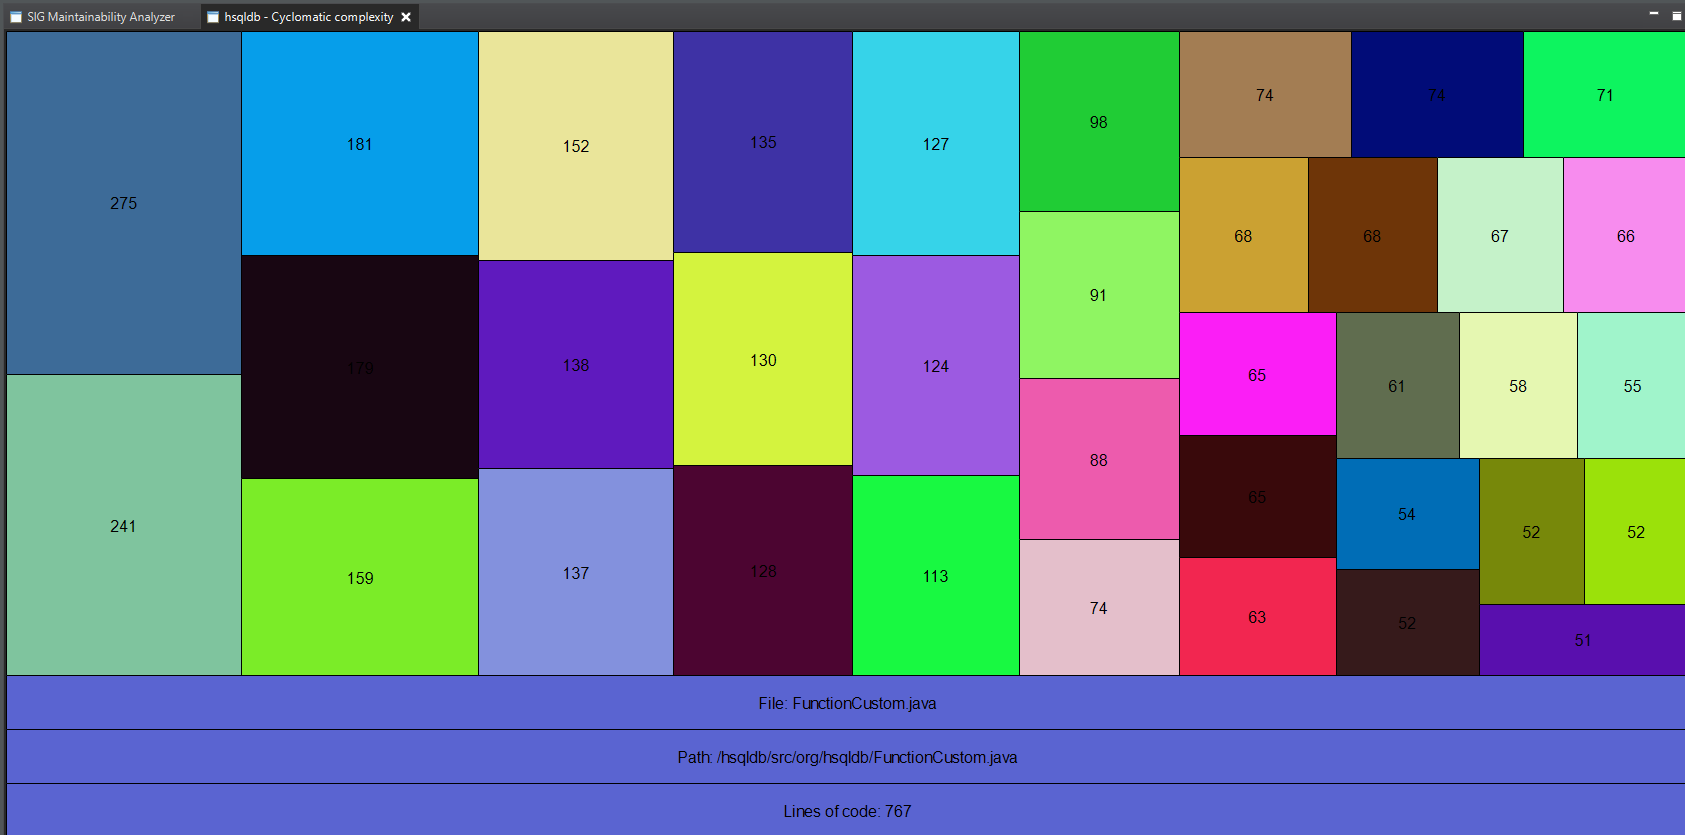
\includegraphics[width=400px, height=200px]{hsqldb_coc.png}
\end{figure}

\clearpage 

Visualizing duplicates is done by combining clones into a single entity. 
We can easily see the amount of clones by counting the amount of boxes per entity.
Of course, we can also navigate to each occurrence of every clone by clicking on the instance.

\begin{figure}[!htbp]
	\centering
	\label{fig:duplication}
	\caption{Fined grained view all duplicates SMALLSQL: Duplication}
	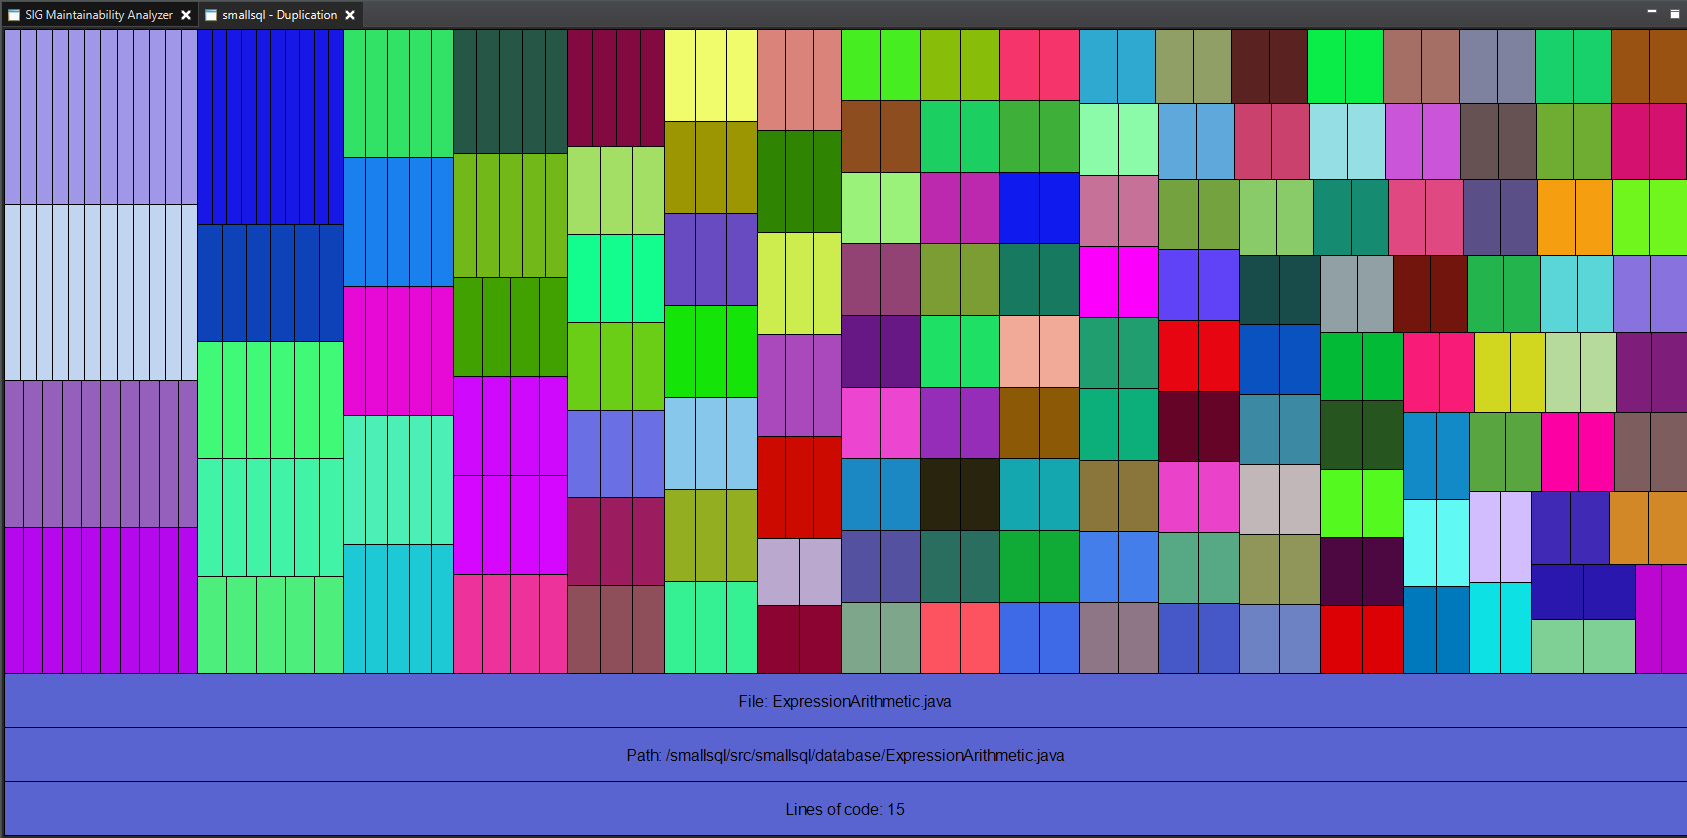
\includegraphics[width=400px, height=200px]{smallsql_duplication.png}
\end{figure}

Note that above screenshots are created using a specific configuration, we can generate different fine-grained views by applying different filters in the menu.

\section{Project Development Stats}

\begin{table}[!htb]
\caption{Project stats}
\begin{tabular}{l|r}	
		\hline
		Files										&			49 \\
		\hline
		Commits										&			130 \\
		\hline
		Feature Branches							&			7 \\
		\hline
		Bugfix Branches								&			1 \\
		\hline
		Other Branches								&			3 \\
		\hline	
		Pull Requests								&			13 \\
		\hline	
		Dives into Rascal source					&			29 \\
		\hline		
		Rascal Documentation Visits					&			1 217 \\ %412 brent-pc 35 brent-lt 770 bas
		\hline		
		Google Searches with 'rascal'				&			78 \\	%57 brent-pc 21 brent-lt
		\hline		
\end{tabular}
\end{table}

\end{document}
